\section{April 4}
\subsection{Field of Moving Charges}
Last time, we concluded with derivation of the components to the \( \mathbf{E} \) field:   
\begin{align*}
	-\nabla V &= \frac{qc}{4 \pi \epsilon_0} \frac{1}{(c \rcurs - \brcurs \cdot \mathbf{v})^2} \left[
	\frac{(c^2 - v^2) \brcurs}{c \rcurs - \brcurs \cdot \mathbf{v}} + \frac{(\mathbf{a} \cdot \brcurs)
\brcurs}{c \rcurs - \brcurs \cdot \mathbf{v}} - \mathbf{v} \right]\\
		-\partial_t \mathbf{A} &= \frac{qc}{4\pi \epsilon_0} \frac{1}{(c \rcurs - \brcurs \cdot \mathbf{v})^2}
	\left[ \frac{\rcurs v^2 - c (\brcurs \cdot \mathbf{v}) - \rcurs (\mathbf{a} \cdot \brcurs)}{c \rcurs -
	\brcurs \cdot \mathbf{v}} \mathbf{v} - \rcurs \mathbf{a} \right]	
\end{align*}
Putting these two together:
\[
	\mathbf{E} = \frac{qc}{4\pi \epsilon_0} \frac{1}{(c\rcurs - \brcurs \cdot \mathbf{v})^3} \left[ (c^2 -
	v^2) \brcurs - \frac{\rcurs}{c}(c^2 - v^2) \mathbf{v} + (\mathbf{a} \cdot \brcurs) \brcurs -
	\frac{\rcurs}{c} (\mathbf{a} \cdot \brcurs) \mathbf{v} - \rcurs^2 \mathbf{a} + \frac{\rcurs}{c}(\brcurs \cdot
	\mathbf{v}) \mathbf{a}\right]
\]
Using some triple cross product magic:
\[
	\mathbf{E} = \frac{1}{4\pi \epsilon_0}\frac{qc}{c \rcurs - \brcurs \cdot \mathbf{v})^3} \left\{ (c^2 -
	v^2) \left( \brcurs - \frac{\rcurs}{c} \mathbf{v} \right) + \brcurs \times \left[ \left( \brcurs -
\frac{\rcurs}{c} \mathbf{v} \right) \times \mathbf{a} \right] \right\}
\]
The first term is called the velocity term, and the second is called the acceleration term. Notice that the
second term in the braces scales as \( \rcurs^2 \), so overall the acceleration term scales as \(
\frac{1}{\rcurs} \). This will become important in chapter 11, when we talk about radiation. With \(
\mathbf{E} \) calculated, we calculate \( \mathbf{B} \):
\[
	\mathbf{B} = \nabla \times \mathbf{A} = \nabla\left( \frac{v}{c^2} V \right) = 
	\frac{1}{c^2}\epsilon^{ijk} \left[ (\partial_j V) v_k  + V \partial_j t_r a_k \right]
\]
working out the cross products and chain rule using the identities we derived in last lecture, we get:
\[
	\mathbf{B} = -\frac{\mu_0}{4\pi} \frac{qc}{(c \rcurs - \brcurs \cdot \mathbf{v})^3} \brcurs \times \left[
	(c^2 - v^2) \mathbf{v} + (\mathbf{a} \cdot \brcurs) \mathbf{v} + (c \rcurs - \brcurs \cdot \mathbf{v})
\mathbf{a} \right]
\]
with some reorganization, it is possible to then find that \( \mathbf{B} = \frac{1}{c} \brcurs \times
\mathbf{E} \), consistent with our earlier conclusion with waveguides. 
Another thing to note is that everything in these equations should be evaluated at the
\textit{retarded time}! That is, \( \rcurs = \mathbf{r} - \mathbf{w}(t_r), \mathbf{v} = \mathbf{v}(t_r), 
\mathbf{a} = \mathbf{a}(t_r) \). 

\begin{example}
	We will explore an application of the formula we just derived by considering a particle that travels at
	constant velocity. We will choose our coordinate system such that the particle travels along the \( x
	\)-axis. A diagram of the situation is as follows:
	\begin{center}
		\begin{tikzpicture}
			\draw[-stealth] (-2, 0) -- (2, 0) node[right] {\( x \)};
			\draw[-stealth] (0, -2) -- (0, 2) node[above] {\( y \)};
			\draw[-stealth, thick, green!80!white] (0, 0) -- (1, 0) node[above] {\( v \)};
		\end{tikzpicture}
	\end{center}
	In this case, we have \( \mathbf{a} = \mathbf{0} \) and \( \mathbf{w}(t) = \mathbf{v}(t) = vt
	\mathbf{\hat{x}} \). Therefore:
	\[
		\brcurs = \mathbf{r} - \mathbf{w}(t_r) = \mathbf{r} - \mathbf{v} t_r
	\]
	and consequently,
	\[
		\brcurs - \frac{\rcurs}{c}\mathbf{v} = \mathbf{r} - \mathbf{v} t_r + (t_r - t) \mathbf{v} =
		\mathbf{r} - \mathbf{v} t \equiv \mathbf{R}
	\]
	Here, we define \( \mathbf{R} \) to be the vector pointing from the charge at the \textit{present} time
	to the field point \( \mathbf{r} \). With this, the \( \mathbf{E} \) field is then:
	\[
		\mathbf{E} = \frac{1}{4\pi \epsilon_0} \frac{qc}{(c \rcurs - \brcurs \cdot \mathbf{v})^3}\left[
		\left( (c^2 - v^2)\left( \brcurs - \frac{\rcurs}{c}\mathbf{v} \right)  \right) \right] =
		\frac{1}{4\pi \epsilon_0} \frac{qc}{(c\rcurs - \brcurs \cdot \mathbf{v})^3} (c^2 - v^2) \mathbf{R}
	\]
	as an exercise, you can show at home that \( c \rcurs - \brcurs \cdot \mathbf{v} = cR\left[ 1 -
	\frac{v^2}{c^2}\sin^2 \theta \right] \), but we will use that result to simplify the above:
	\[
		\mathbf{E} = \frac{q}{4\pi \epsilon_0} \frac{\mathbf{\hat{R}}}{R^2} \frac{\left( 1 - \frac{v^2}{c^2}
		\right)}{\left( 1 - \frac{v^2}{c^2} \sin^2 \right)^{3 / 2}}
	\]
	Now, notice that the direction is determined by \( \mathbf{R} \), which means that the field direction of
	is given by the position of the particle in \textit{present time}, not retarded time! In addition,
	because of the \( \sin \theta \) factor in the denominator, it means that the \( \mathbf{E} \) gets
	stronger as \( \theta \to \frac{\pi}{2} \), and the field lines "squeeze" closer in that direction. This
	is better illustrated via a diagram:
	\begin{center}
		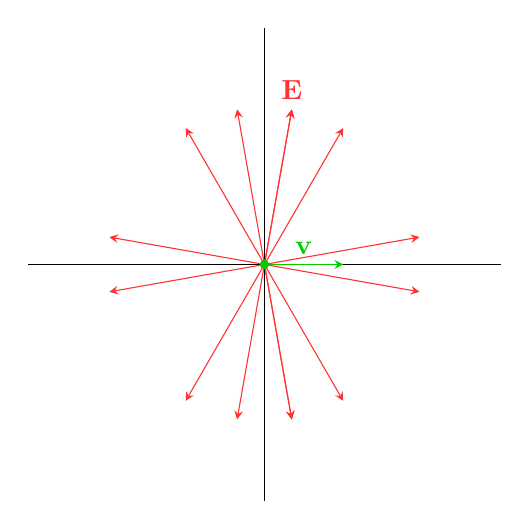
\begin{tikzpicture}
			\draw (-3, 0) -- (3, 0);
			\draw (0, -3) -- (0, 3);
			\draw[green!80!black, -stealth] (0, 0) -- (1, 0) node[midway, above] {\( \mathbf{v} \)};

			% horizontal lines
			\draw[-stealth, red!80!white] (0, 0) -- (10:2);
			\draw[-stealth, red!80!white] (0, 0) -- (-10:2);
			\draw[-stealth, red!80!white] (0, 0) -- (-170:2);
			\draw[-stealth, red!80!white] (0, 0) -- (170:2);
			
			% vertical lines
			\draw[-stealth, red!80!white] (0, 0) -- (80:2) node[above] {\( \mathbf{E} \)};
			\draw[-stealth, red!80!white] (0, 0) -- (-80:2);
			\draw[-stealth, red!80!white] (0, 0) -- (280:2);
			\draw[-stealth, red!80!white] (0, 0) -- (-280:2);
			\draw[-stealth, red!80!white] (0, 0) -- (260:2);
			\draw[-stealth, red!80!white] (0, 0) -- (-260:2);
			\draw[-stealth, red!80!white] (0, 0) -- (60:2);
			\draw[-stealth, red!80!white] (0, 0) -- (120:2);
			\draw[-stealth, red!80!white] (0, 0) -- (-60:2);
			\draw[-stealth, red!80!white] (0, 0) -- (-120:2);

			\filldraw[green!80!black] (0, 0) circle (0.05);
		\end{tikzpicture}
	\end{center}
	As for the \( \mathbf{B} \) field, we know that \( \mathbf{B} = \frac{1}{c}\hat{\brcurs} \times
	\mathbf{E} \), so:
	\[
		\mathbf{B} = \frac{1}{c} \frac{\brcurs}{\rcurs} \times \mathbf{E} = \frac{1}{c \rcurs} \left(
		\mathbf{R} + \frac{\rcurs}{c} \mathbf{v} \right) \times \left( \frac{q}{4\pi \epsilon_0}
	\frac{\mathbf{\hat{R}}}{R^2} \frac{1 - v^2 / c^2}{(1 - \frac{v^2}{c^2}\sin^2 \theta)^{3 / 2}} \right)
	\]
	Becuase \( \mathbf{\hat{R}} \times \mathbf{\hat{R}} = \mathbf{0} \), only the second term survives. This
	gives us a \( \mathbf{B} \) field that circles around the particle:
	\begin{center}
		\begin{tikzpicture}[decoration={markings,mark=at position 0.5 with {\arrow{stealth}}}]
			\draw[thick,-stealth] (-2,0) -- (2.5,0) node[right] {$x$};
			\draw[thick,stealth-stealth] (0,-1.5) -- (0,1.5) node[left] {$y$};
			\draw[very thick,green!70!blue!50,-stealth] (0,0) -- (0.75,0) node[below] {$\vec{v}$};
			\filldraw[green!70!blue!50] (0,0) circle (0.05cm);
			\draw[thick,orange!70!white,postaction={decorate}] (0,0) ellipse (-0.25cm and 1cm);
			\filldraw[white] (-0.3,0.125) rectangle (-0.2,-0.125);
			\draw[thick] (-0.31,0) -- (-0.19,0);
			\draw[thick,orange!70!white,postaction={decorate}] (-1.5,0) ellipse (-0.1cm and 0.4cm);
			\filldraw[white] (-1.65,0.125) rectangle (-1.55,-0.125);
			\draw[thick] (-1.66,0) -- (-1.54,0);
			\draw[thick,orange!70!white,postaction={decorate}] (1.5,0) ellipse (-0.1cm and 0.4cm);
			\filldraw[white] (1.35,0.125) rectangle (1.45,-0.125);
			\draw[thick] (1.34,0) -- (1.46,0);
		\end{tikzpicture}
	\end{center}
	We also talked about an intuitive way to think about this, called the \textbf{Thomson Kink Model}. To be
	completely honest, I can't explain this part of it better than Griffiths does, so just read examples 10.4
	and 10.5 there for a better description. 
\end{example}
